\documentclass{article}
\usepackage[utf8]{inputenc}
\usepackage[english]{babel}
\usepackage{graphicx}
\usepackage{color}
\usepackage{amsfonts}

\def\warning#1{\color{red} #1 \color{black}}
\def\note#1{\color{cyan} #1 \color{black}}
\def\circled#1{\raisebox{.5pt}{\textcircled{\raisebox{-.9pt} {#1}}}}

\begin{document}

\title{Examen Discrete Wiskunde 22 januari 2018}
\date{}
\author{}
\maketitle

\note{Het percentageteken voor elke vraag wijst op de relatieve score van die vraag}

\begin{enumerate}
\item {\note{10\%} Gebruik de Baby-step, Giant-step techniek om de index van 12 ten opzichte van de primitieve wortel $\omega = 3$ in ($\mathbb{Z}_{46049}, \cdot$) te berekenen. Gebruik hierbij giant-steps van 200 baby-steps groot. Vermeld ook het aantal giant-steps en de extra baby-steps die nodig zijn. Een oplossing louter gebaseerd op het berekenen van de opeenvolgende machten van $\omega$, wordt als waardeloos beschouwd.}
\item {\note{5\%} Van welke graaf {\bf G} is de hieronder getekende graaf de lijngraaf. Maak een figuur van de graaf {\bf G} en geef de staandaardidentificatie (naam en symbool).

    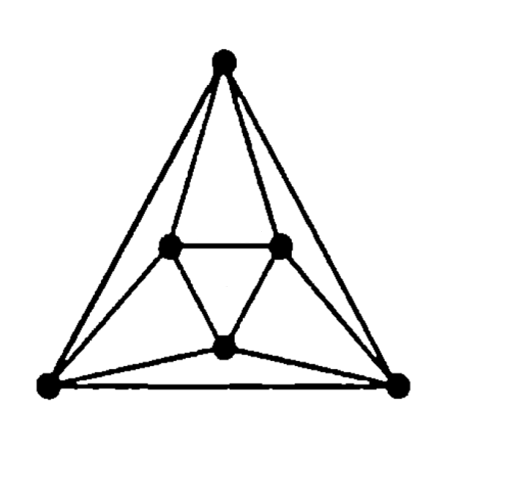
\includegraphics[width=5cm]{lijngraaf}}

\item {\note{20\%} Beschouw het veld $F_{16}$ en de elliptische kromme E: $y^2+xy = x^3 + \circled{3}x^2 + \circled{5} $ over dit veld. De irreducibele veelterm is $\mu = x^4 + x + 1$ en de primitieve wortel $\omega = x$. Gebruik de onderstaande groepstabel (\warning{todo: groepstabel})

    \begin{itemize}
    \item {\note{8\%} Het punt $A(x + 1, x^3)$ is één van de punten van de elliptische kromme E. Bepaal alle andere punten en duid hierbij aan welke inversen zijn van elkaar. Hoeveel punten heeft deze elliptische kromme?}
    \item {\note{6\%} Bereken 2A, 4A en 8A en identificeer het resultaat met één van de hiervoor gevonden punten.}
      \item {\note{6\%} Bereken de overige veelvouden van A, tot je hetzij het neutrale element, hetzij het punt dat zijn eigen inverse is bekomt. Bepaal hieruit de structuur van de overeenkomstige groep. Is de groep cyclisch en zo ja, met hoeveel primitieve elementen.}

      \end{itemize}}

  \item {\note{10\%} Welk criterium moet, of welke criteria moeten voldaan zijn opdat een veelterm irreducibel is. Ga na of $x^5 + x^4 + 2x^3 +2x + 1$ hieraan voldoet.}
  \item {\note{15\%} \warning{Stapelprobleem met Excel (Veralgemeende algoritme X toepassen. Ongeveer 50 kolommen en 2000 rijen, 21 soepele voorwaarden, 32 stricte voorwaarden)}}
  \item {\note {12\%} Teken het cykeldiagram van de groep, waarvan de groepstabel hieronder gegeven is. Bepaal vervolgens de partitionering van de groepselementen in conjugatieklassen. Stel tenslotte de conjugatievergelijking op. 
      \begin{tabular}{|c|c|c|c|c|c|c|c|c|c|c|c|c|c|c|c|}

        % ACEGIKMO
        % BDFHJLNP
        \hline
        A&B&C&D&E&F&G&H&I&J&K&L&M&N&O&P \cr \hline
        B&A&D&C&F&E&H&G&J&I&L&K&N&M&P&O \cr \hline
        C&H&E&J&G&L&I&N&K&P&M&B&O&D&A&F \cr\hline
        D&G&F&I&H&K&J&M&L&O&N&A&P&C&B&E \cr\hline
        E&N&G&P&I&B&K&D&M&F&O&H&A&J&C&L \cr\hline
        F&M&H&O&J&A&L&C&N&E&P&G&B&I&D&K \cr\hline
        G&D&I&F&K&H&M&J&O&L&A&N&C&P&E&B \cr\hline
        H&C&J&E&L&G&N&I&P&K&B&M&D&O&F&A \cr\hline
        I&J&K&L&M&N&O&P&A&B&C&D&E&F&G&H \cr\hline
        J&I&L&K&N&M&P&O&B&A&D&C&F&E&H&G \cr\hline
        K&P&M&B&O&D&A&F&C&H&E&J&G&L&I&N \cr\hline
        L&O&N&A&P&C&B&E&D&G&F&I&H&K&J&M \cr\hline
        M&F&O&H&A&J&C&L&E&N&G&P&I&B&K&D \cr\hline
        N&E&P&G&B&I&D&K&F&M&H&O&J&A&L&C \cr\hline
        O&L&A&N&C&P&E&B&G&D&I&F&K&H&M&J \cr\hline
        P&K&B&M&D&O&F&A&H&C&J&E&L&G&N&I \cr\hline
      \end{tabular}

    }

  \item {\begin{itemize}
      \item {\note{12\%} Bepaal de cykelindex om de hoekpunten van een reguliere achthoekige ster (Stellated Octahedron), waarbij zowel rotaties als spiegelingen in beschouwing worden genomen. Je kan deze figuur manipuleren door het programma Antiview op te starten met het argument UC4. (.\\antiview.exe UC4)}
      \item {\note{10\%} Hoeveel configuraties zijn er mogelijk waarbij er 2 kleuren 4 maal gebruikt worden. Hoeveel van deze configuraties zijn een spiegelbeeld van elkaar?}
        \item {\note{6\%} Hoeveel configuraties zijn er mogelijk waarbij er 4 kleuren 2 maal gebruikt worden. Hoeveel van deze configuraties zijn een spiegelbeeld van elkaar?}
      \end{itemize}}
\end{enumerate}



\end{document}


% green 147 BLUE 240